%%%%%%%%%%%%%%%%%%%%%%%%%%%%%%%%%%%%%%%%%%%%%%%%%%%%%%%%%%%%%%%%%%%%%%%
%\vspace*{170mm}
% Lage eps fra Excel::
% 1. I Excel: Print Tabellsiden til PDF-fil via Distiller. 
%    (Distiller, Ikke avkryss "Do not send fonts to distiller" i Properties|Settings ved print)
%    (Evt. print via PS-fil, så "Send To: Distiller"
% 2. Åpne i Acrobat Reader, Save As: Type=EPS, 
%     Settings|General:
%               Ascii
%               Font Inclusion: Embedded and referenced fonts
%               Ikke kryss  "Clip to bounding box"
%               Ikke kryss  "Include Preview"
%
%%%%%%%%%%%%%%%%%%%%%%%%%%%%%%%%%%%%%%%%%%%%%%%%%%%%%%%%%%%%%%%%%%%%%%%
\documentclass[../Elmag-labhefte-2020.tex]{subfiles}
\begin{document}


\setchapterpreamble[u]{\margintoc}
\chapter{STATIC MAGNETIC FIELD \label{ch.magnetfelt}}

\subsection*{Goal}

In this lab assignment you will
%
\begin{itemize}
    \item develop your skills in documenting laboratory work with the lab journal,
    \item set up and carry out physical measurements,
    \item perform basic error analysis,
    \item learn to measure magnetic fields with Hall effect gaussmeter,
    \item study the magnetic field around a short coil, Helmholtz coil and solenoid,
    %\item bli kjent med feltbegrepet i fysikken 
    \item use Python or Excel spreadsheets to compare calculated and measured results.
\end{itemize}
%

%**********************************************
\section{Theoretical background}
%**********************************************

Biot-Savart's law is presented here. Some theory is presented in the text for the calculation tasks in section \ref{ch.magnetfelt.beregn}. Otherwise, reference is made to the textbook and the lectures in electromagnetism.

\subsection{Biot-Savart's Law}

Electric fields are generated around any electric charge while magnetic fields are generated around electric charges that move. In 1820, Jean-Baptiste Biot and Félix Savart performed magnetic field experiments on live conductors and set up the following expression for the magnetic field contribution $\dd{\va*{B}}$ at a point P in space from the current $I$ in a wire element $\dd{\va*{s}}$,
\begin{equation}
    \dd{\va*{B}} = \frac{\mu_0}{4\pi} \frac{I \dd{\va*{s}} \cross \vu{r}}{r^2} ,
    \label{eq:Biot.Savart}
\end{equation}
where $\va*{r}$ is the position vector of the point P measured from the current element $I \dd{\va*{s}}$, $\vu{r} = \va*{r}/r$ is the unit vector along $\va*{r}$ and $\mu_0$ is the magnetic permeability in empty space. Note the $r^{-2}$ dependence, the same as for the electric field strength in Coulomb's law. The superposition principle applies to magnetic fields, and consequently the total field strength $\va*{B}$ at point P from the whole conductor can be found by integrating over the length $s$ of the conductor:
\begin{equation}
    \va*{B}(\va*{r}) = \frac{\mu_0 I}{4 \pi} \int_s \frac{ \dd{\va*{s}} \cross \vu{r}} {r^2} .
    \label{eq:Biot.Savart2}
\end{equation}
%
In the experiment, you will examine the magnetic field along the axis of circular coils. The simplest circular spool you can make consists of a simple wire loop as shown in Figure \ref{magnetfelt.fig1}.

\begin{figure}[!ht]
    \setlength{\unitlength}{0.6mm}
    \begin{picture}(177,90)(0,-20)
        \linethickness{0.3mm}
        \qbezier(30, 60)(11, 58.5)(9,30)
        \qbezier(9, 30)(8, 3)(24,2) 
        \qbezier(30, 60)(45, 58.5)(46,30)
        \qbezier(46, 30)(44, 6)(28,2)
        \qbezier(35, 2)(44, 8)(46,16)
        \put(46,16){\vector(0,1){1}}
        \qbezier(19, -20)(21.5, -9)(24,2)
        \qbezier(23, -20)(25.5, -9)(28,2)
        \put(30,30){\line(0,1){30}}
        \qbezier(30, 30)(35, 42)(40,54)
        \qbezier(30, 45)(34, 46)(35,42)
        \put(30,60){\line(4,-1){120}} 
        \multiput(30,30)(2,0){60}{\line(1,0){1}}
        \put(30,60){\vector(4,-1){10}}
        \put(30.1,60.1){\vector(4,-1){10}}
        \put(29.9,59.9){\vector(4,-1){10}}
        \put(30,60){\vector(-1,0){6}}
        \put(26,62){\makebox(0,0)[b]{\large$\dd{\va*{s}}$}}
        \put(26,62){\makebox(0,0)[b]{\large$\dd{\va*{s}}$}}
        \put(36,60){\makebox(0,0)[b]{\large$\vu{r}$}}
        \put(76,50){\makebox(0,0)[b]{\large$r$}}
        \put(76,25){\makebox(0,0)[b]{\large$x$}}
        \put(116,32.5){\makebox(0,0)[b]{\large$\alpha$}}
        \put(26,42){\makebox(0,0)[b]{\large$\xi$}}
        \put(42,2){\makebox(0,0)[b]{\large$I$}}
        \put(30,-12){\makebox(0,0)[b]{\large$I$}}
        \qbezier(120, 30)(119, 35)(122,37)  
        \put(27,-12){\vector(1,4){3}}
        \put(21,0){\vector(-1,-4){3}} 
        \put(150,30){\vector(1,0){10}}
        \put(150,30){\vector(0,1){20}}
        \put(150,30){\vector(1,2){10}}
        \color{black}
        \qbezier(150, 42)(153, 43)(155,40)
        \put(150,23){\makebox(0,0)[b]{\large P}}
        \put(167,27){\makebox(0,0)[b]{\large$\dd{B_x}$}}
        \put(146,52){\makebox(0,0)[b]{\large$\dd B_\perp$}}
        \put(165,50){\makebox(0,0)[b]{\large$\dd \va*{B}$}}
        \put(153,44){\makebox(0,0)[b]{\large$\alpha$}}
        \put(33,46){\makebox(0,0)[b]{\large$\theta$}}
        \put(31,45.1){\vector(-1,0){1}}
        \thinlines
        \multiput(160,30)(0,2){10}{\line(0,1){1}}
        \multiput(150.5,50)(2,0){5}{\line(1,0){1}}
    \end{picture}
    \caption{The magnetic field on the normal axis of a circular coil.}
    \label{magnetfelt.fig1}
\end{figure}

The magnetic field on the axis of the coil will have a component in the axis direction $x$ and a component normal to this. According to Biot-Savart's law, the normal component will be zeroed out by contributions (integration) over the entire loop, as the symmetry of the system gives equal strength in all directions. For the $x$ component we get by inserting $r^2 = x^2 + \xi^2$ and using $\sin \alpha = \xi/r$,
%
\begin{align}
    \dd{B_x} &= \frac{\mu_0 I}{4 \pi} \frac{\dd{s}}{x^2 + \xi^2} \sin\alpha \nonumber \\
             &= \frac{\mu_0 I}{4 \pi}  \frac{\xi \dd{\theta}}{x^2 + \xi^2}  \frac{\xi}{\sqrt{x^2 + \xi^2}} ,
\end{align}
where $\theta$ is the integration angle around the loop circle. Integrated over the loop with $\int \dd{\theta} = 2\pi$ gives this result
%
\begin{equation} 
    \label{eq:Biot.Savart3}
    B_x = \frac{\mu_0 I}{4 \pi} \frac{2\pi \xi^2}{\left( x^2 + \xi^2 \right)^{3/2}}
        = \frac{\mu_0 I}{2 \xi} \qty(1 + \frac{x^2}{\xi^2})^{-3/2}.
\end{equation}
For $x = 0$ (middle of the loop) this gives $B_x = \flatfrac{\mu_0 I}{2\xi}$ and for $x \gg \xi$ (far away from the loop), $B_x = \flatfrac{\mu_0 I\xi^2}{2x^3}$.


%%%%%%%%%%%%%%%%%%%%%%%%%%%%%%%%%%%%%%%%%%%%%%%%%%%
\section{Calculation tasks \label{ch.magnetfelt.beregn}}
%%%%%%%%%%%%%%%%%%%%%%%%%%%%%

%%%%%%%%%%%%%%%%%%%%%%%%%%%%%%%%%%%%%%%%%%%%%%%%%%%%%%%%%%%%%%%%%%%%%%%%%%%%%%
\subsection{Calculation and documentation \label{ch.magnetfelt.regneark}}
%%%%%%%%%%%%%%%%%%%%%%%%%%%%%%%%%%%%%%%%%%%%%%%%%%%%%%%%%%%%%%%%%%%%%%%%%%%%%%

To perform calculations and to create tables / diagrams, you can freely choose between suitable programs (for example Python, Matlab, Origin, Excel or similar). Data and results must be documented in the lab journal (for example by pasting printouts of the tables and diagrams in the lab journal or by writing the results by hand). The source code and the original files used for calculation must be available in case of questions. The source code can be pasted into the lab journal.

\subsection{Short Coil}

The magnetic field from a short coil with $N$ windings can be considered far from the coil (in relation to the extent of the coil) as the sum of the magnetic field from $N$ current loops given in equation \eqref{eq:Biot.Savart3}. The magnetic field on the axis at a distance $x$ from the mean center
\sidenote{Recall that the coils have finite thickness, so we use the mean center.}
of the coil is then according to equation \eqref{eq:Biot.Savart3} given by
%
\begin{equation}
    B(x) = \frac{N\mu_0 I}{2 R} \qty(1 + \frac{x^{2}}{R^{2}})^{-3/2},
    \label{eq:kort.spole}
\end{equation}
%
where $R$ is the average radius of the current loops.

Assume that you have a short coil with $N = \SI{330}{\windings}$ and an average radius $\langle R \rangle  = \SI{70}{\mm}$ with a constant current $I = \SI{1.00}{\ampere}$ through the windings.

\emph{1A. Make a table of the magnetic flux density $B(x)$ on the axis of the coil in the area $-\SI{20}{\cm} < x < \SI{20}{\cm}$.}

A suggested table is shown in Table \ref{tab:example-table}.
Constants are entered in rows under the heading.
\begin{table}[th]
  \caption{Calculated and measured values of the magnetic field $B$ along the axis of a short coil as a function of the distance $x$ from the center of the coil.\label{tab:example-table}}
  \begin{tabular}{lrl}
    \hline
    Magnetic permeability for vacuum, $\mu_0$ & 1.26E-0.6 & H/m\\
    Number of windings, $N$ & 330 & \#\\
    Current, $I$ & 1.00 & A\\
    Average loop radius, $R$ & 0.07 & m\\
    \hline
  \end{tabular}
  
  \vspace{1em}
  \begin{tabular}{rrrrr}
    \hline\\
    \thead{Position} & \thead{$x$} & \thead{Calculated} & \thead{Measured} & \thead{Difference}\\
    \thead{(cm)} & \thead{(m)} & \thead{(gauss = $10^{-4}T$)} & \thead{(gauss)} & \thead{(\%)}\\
    \hline
    24.5 & -0.25 & 0.581 &  & -100.0\\
    29.5 & -0.2 & 1.068 &  & -100.0\\
    34.5 & -0.15 & 2.241 &  & -100.0\\
    39.5 & -0.10 & 5.588 &  & -100.0\\
    44.5 & -0.05 & 15.965 &  & -100.0\\
    47.5 & -0.02 & 26.339 &  & -100.0\\
    48.5 & -0.01 & 28.745 &  & -100.0\\
    49.5 & 0.00 & 29.629 &  & -100.0\\
  \end{tabular}
\end{table}

%% Written in Emacs orgtbl 

\begin{comment}
% BEGIN RECEIVE ORGTBL extabell
\begin{tabular}{rrrlr}
24.5 & -0.25 & 0.581 &  & -100.0\\
29.5 & -0.2 & 1.068 &  & -100.0\\
34.5 & -0.15 & 2.241 &  & -100.0\\
39.5 & -0.10 & 5.588 &  & -100.0\\
44.5 & -0.05 & 15.965 &  & -100.0\\
47.5 & -0.02 & 26.339 &  & -100.0\\
48.5 & -0.01 & 28.745 &  & -100.0\\
49.5 & 0.00 & 29.629 &  & -100.0\\
\end{tabular}
% END RECEIVE ORGTBL extabell
#+ORGTBL: SEND extabell orgtbl-to-latex :splice nil :skip 0
| 24.5 | -0.25 |  0.581 |   | -100.0 |
| 29.5 |  -0.2 |  1.068 |   | -100.0 |
| 34.5 | -0.15 |  2.241 |   | -100.0 |
| 39.5 | -0.10 |  5.588 |   | -100.0 |
| 44.5 | -0.05 | 15.965 |   | -100.0 |
| 47.5 | -0.02 | 26.339 |   | -100.0 |
| 48.5 | -0.01 | 28.745 |   | -100.0 |
| 49.5 |  0.00 | 29.629 |   | -100.0 |
\end{comment}


% \begin{figure}[!ht]
% \RawFloats
%     \begin{center}
%     %\vspace{25mm}
%     %magnetfelt.tab1
%     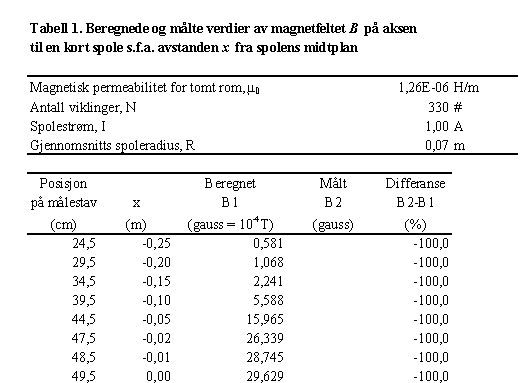
\includegraphics[scale=0.9]{fig/magnetfelt-tab1.png}

%     \end{center}
%     \caption{%
%         Utdrag fra en Excel-tabell for magnetfelt på aksen til tynn spole.
%     }
%     \label{magnetfelt.tab1}
% \end{figure}
%\emph{Hjelp:} Dersom f.eks. første tallinje i tabellen er skrevet inn på rad 14 og beregnet verdi er i kolonne 3 vil formelen som representerer likning \eqref{eq:kort.spole}  bli slik: \\[3mm]
%\verb" =(($E$4*$E$5*$E$6)/(2*$E$7))*((1+(B14/$E$7)^2)^(-1,5))*10000".
%\\[3mm]
%Verdien er multiplisert med \num{10000} slik at $B(x)$ vises i \si{\gauss} (\SI{e-4}{\tesla}), som er tallverdiene gaussmeteret viser. 

\emph{1B. Present the result in a graph.}

\emph{Discuss the calculation of the magnetic field of a short coil when the extent of the coil is taken into account.}

The program or spreadsheet in Excel can also be used to calculate expected magnetic field strengths as a result of Biot-Savart's \eqref{eq:Biot.Savart3} law and subsequent comparison with experimentally measured magnetic field strengths in section \ref{ch.magnetfelt.eksperimentelt}.

\emph{1C. Include a column for measured value of $B$ and a column for deviation between measured and calculated value given in \si{\percent}, and also prepare to show the deviation graphically.} (A suggestion is given in Table \ref{tab:example-table}.)

Calculate also one of the values of $B$ by hand, and verify the value of the difference between calculated and measured.

\vspace{4mm}

\emph{A small challenge for those with extra time:}

The actual spool you are going to use in the problem has 22 windings in 15 layers with an effective wire diameter equal to \SI{0.93}{\mm}, wound with inner diameter equal to \SI{126}{\mm} and outer diameter equal to \SI{154}{\mm}.

\emph{2. How do you think the real magnetic field near the coil will differ from the magnetic field calculated from equation \eqref{eq:kort.spole}?}
\sidenote{TIP: Look at the extent of the coil as an error in $x$ and estimate the corresponding error $\Delta B$ in $B(x)$.}

\emph{3. If you were to take into account the extent of the coil during the calculations of the field, how would you proceed?} \sidenote{TIP: Divide the coil into e.g. three coils with 110 windings each and calculate the field from each of the coils and superimpose the effect. The best thing you can do is treat each winding separately, and in practice, that means integration over each winding.}

\subsection{Helmholtz coils}
%%%%%%%%%%%%%%%%%%%%%%%%%%%%%%%%%%%%%%%%%%%%%%%%%%%%%%

So-called Helmholtz coils
%\footnote{Oppkalt etter Hermann Ludwig Ferdinand von Helmholtz (1821-1894), tysk medisiner og fysiker.} 
\sidenote{Named after Hermann Ludwig Ferdinand von Helmholtz (1821-1894), German physicist and physician.}
consist of two identical, short coils connected in series set up concentrically at a distance $a$ as shown in figure \ref{magnetfelt.fig2}. The axial magnetic field on the axis is given by equation \eqref{eq:kort.spole} for each coil. According to the superposition principle, we find the total field at a distance $x$ from the center plane between the coils to be equal
%
\begin{equation}
    B_x (x) 
        = \frac{N \mu_0 I}{2 R} \qty[\qty(1 + \frac{(x - \flatfrac{a}{2})^2}{R^2})^{-3/2} 
            + \qty(1 + \frac{(x + \flatfrac{a}{2})^2}{R^2})^{-3/2}].
    \label{eq:Helmholtz}
\end{equation}
%
Here the average radius of the coils is equal to $R$, the current through the coils is equal to $I$ and we have neglected the extent of the coils.

If you differentiate equation \eqref{eq:Helmholtz} with respect to $x$ you will find that at $x = 0$ the derivatives
\[
  \dv{B}{x} = \dv[2]{B}{x} = \dv[3]{B}{x} = 0
\]
when $a = R$. This means that when $a = R$ you have a geometry that gives you a particularly good homogeneous magnetic field in the area between the coils. Such Helmholtz coils are used to set up homogeneous magnetic fields in many situations.

\begin{marginfigure}[-2cm]%[!ht]
    \setlength{\unitlength}{0.6mm}
    \begin{picture}(120,80)(30,0)
        \linethickness{0.5mm}
        \put(44,79){\makebox(0,0)[b]{\large$\bigodot$}}
        \put(44,19){\makebox(0,0)[b]{\large$\bigoplus$}}
        \put(40,19){\framebox(8,8)}%[20,20]{KRN}
        \put(40,79){\framebox(8,8)}%[20,60]{KRN}
        \put(104,79){\makebox(0,0)[b]{\large$\bigodot$}}
        \put(104,19){\makebox(0,0)[b]{\large$\bigoplus$}}
        \put(100,19){\framebox(8,8)}%[20,20]{KRN}
        \put(100,79){\framebox(8,8)}%[20,60]{KRN}
        \put(74,47){\line(0,1){6}} 
        \put(30,50){\vector(1,0){100}} %x-axis
        %\qbezier(128, 51)(129, 50.5)(130,50)
        %\qbezier(128, 49)(129, 49.5)(130,50)
        
        \qbezier(126, 51.5)(128, 50.8)(130,50)
        \qbezier(126, 49)(128, 49.5)(130,50)
        
        %\color{magenta}
        \put(44,60){\line(1,0){60}} 
        \qbezier(47, 61)(47, 61)(44,60)
        \qbezier(47, 59)(47, 59)(44,60)
        \qbezier(102, 61)(102, 61)(104,60)
        \qbezier(102, 59)(102, 59)(104,60)
        %%\color{yellow}
        \thinlines
        \put(39.7,27.8){\framebox(8.4,51)}%[20,60]{KRN}
        \put(99.7,27.8){\framebox(8.4,51)}%[20,60]{KRN}
        \put(134,48){\makebox(0,0)[b]{\large$x$}}
        \put(74,62){\makebox(0,0)[b]{\large$a$}}
        \put(74,40){\makebox(0,0)[b]{\large O}}
        \put(26,64){\makebox(0,0)[b]{\large$R$}}
        \put(68,20){\makebox(0,0)[b]{\small\sf Windings}}
        \put(32,50){\vector(0,1){32}}
        %%\color{magenta}
        \put(55,22){\vector(-1,-0){5}} 
    \end{picture}
    \caption{%
        Helmholtz coils consist of to thin concentric coils at a distance $a$ from each other.
    }
    \label{magnetfelt.fig2}
\end{marginfigure}
Suppose you have Helmholtz coils with $N = \SI{330}{\windings}$ on each coil, $R = \SI{70}{\mm}$ and send a constant current $I = \SI{1.00}{\ampere}$ through the windings.

\emph{4A. Make a table of the magnetic flux density $B(x)$ on the axis of the Helmholtz coil in the range $\SI{-20}{\cm} < x < \SI{20}{\cm}$ for each of the three different values   $a = R/2, R$ and $2R$.}

A suggested table is shown in Table \ref{tab:example-table2}.

\begin{table*}[h]
  \tiny
  \caption{Calculated and measured values of the magnetic field $B$ along the axis of a Helmholtz coil as a function of the distance $x$ from the center of the coil, for different values of the separation $a$.\label{tab:example-table2}}
  \begin{tabular}{l rl}
    \hline
    Magnetic permeability for vaccum, $\mu_0$ & 1.26E-0.6 & H/m\\
    Number of windings, $N$ & 330 & \#\\
    Current, $I$ & 1.00 & A\\
    Average loop radius, $R$ & 0.07 & \\
    \hline
  \end{tabular}
  
  \vspace{1em}
  \begin{tabular}{rr|rrr|lrl|rlr}
    \hline
    && \multicolumn{3}{c}{$a=2R$}& \multicolumn{3}{c}{$a=2R$}& \multicolumn{3}{c}{$a=2R$}\\
    Position& $x$ & Calculated & Measured & Difference& Calculated & Measured & Difference& Calculated & Measured & Difference\\
    (cm) & (m) & (gauss) & (gauss) & (\%) & (gauss) & (gauss) & (\%) & (gauss) & (gauss) & (\%)\\
    \hline
    30 & -0.20 & 3.626 &  & -100 & 2.454 &  & -100 & 2.213 &  & -100\\
    35 & -0.15 & 9.286 &  & -100 & 5.478 &  & -100 & 4.719 &  & -100\\
    40 & -0.10 & 24.643 &  & -100 & 14.549 &  & -100 & 11.996 &  & -100\\
    43 & -0.07 & 32.279 &  & -100 & 26.258 &  & -100 & 22.393 &  & -100\\
    45 & -0.05 & 30.129 &  & -100 & 35.312 &  & -100 & 33.160 &  & -100\\
    47 & -0.03 & 24.981 &  & -100 & 41.063 &  & -100 & 45.054 &  & -100\\
    48 & -0.02 & 22.821 &  & -100 & 42.105 &  & -100 & 49.866 &  & -100\\
    49 & -0.01 & 21.429 &  & -100 & 42.382 &  & -100 & 53.017 &  & -100\\
    50 & 0.00 & 20.951 &  & -100 & 42.402 &  & -100 & 54.108 &  & -100\\
    \hline
  \end{tabular}
\end{table*}

% % BEGIN RECEIVE ORGTBL magtbl2
% \begin{tabular}{rrrlrrlrrlr}
% 30 & -0.20 & 3.626 &  & -100 & 2.454 &  & -100 & 2.213 &  & -100\\
% 35 & -0.15 & 9.286 &  & -100 & 5.478 &  & -100 & 4.719 &  & -100\\
% 40 & -0.10 & 24.643 &  & -100 & 14.549 &  & -100 & 11.996 &  & -100\\
% 43 & -0.07 & 32.279 &  & -100 & 26.258 &  & -100 & 22.393 &  & -100\\
% 45 & -0.05 & 30.129 &  & -100 & 35.312 &  & -100 & 33.160 &  & -100\\
% 47 & -0.03 & 24.981 &  & -100 & 41.063 &  & -100 & 45.054 &  & -100\\
% 48 & -0.02 & 22.821 &  & -100 & 42.105 &  & -100 & 49.866 &  & -100\\
% 49 & -0.01 & 21.429 &  & -100 & 42.382 &  & -100 & 53.017 &  & -100\\
% 50 & 0.00 & 20.951 &  & -100 & 42.402 &  & -100 & 54.108 &  & -100\\
% \end{tabular}
% % END RECEIVE ORGTBL magtbl2
\begin{comment}
#+ORGTBL: SEND magtbl2 orgtbl-to-latex :splice nil :skip 0
| 30 | -0.20 |  3.626 |   | -100 |  2.454 |   | -100 |  2.213 |   | -100 |
| 35 | -0.15 |  9.286 |   | -100 |  5.478 |   | -100 |  4.719 |   | -100 |
| 40 | -0.10 | 24.643 |   | -100 | 14.549 |   | -100 | 11.996 |   | -100 |
| 43 | -0.07 | 32.279 |   | -100 | 26.258 |   | -100 | 22.393 |   | -100 |
| 45 | -0.05 | 30.129 |   | -100 | 35.312 |   | -100 | 33.160 |   | -100 |
| 47 | -0.03 | 24.981 |   | -100 | 41.063 |   | -100 | 45.054 |   | -100 |
| 48 | -0.02 | 22.821 |   | -100 | 42.105 |   | -100 | 49.866 |   | -100 |
| 49 | -0.01 | 21.429 |   | -100 | 42.382 |   | -100 | 53.017 |   | -100 |
| 50 |  0.00 | 20.951 |   | -100 | 42.402 |   | -100 | 54.108 |   | -100 |
\end{comment}


% \begin{figure}[!ht]
% \RawFloats
%     \begin{center}
%     %\vspace{25mm}
%     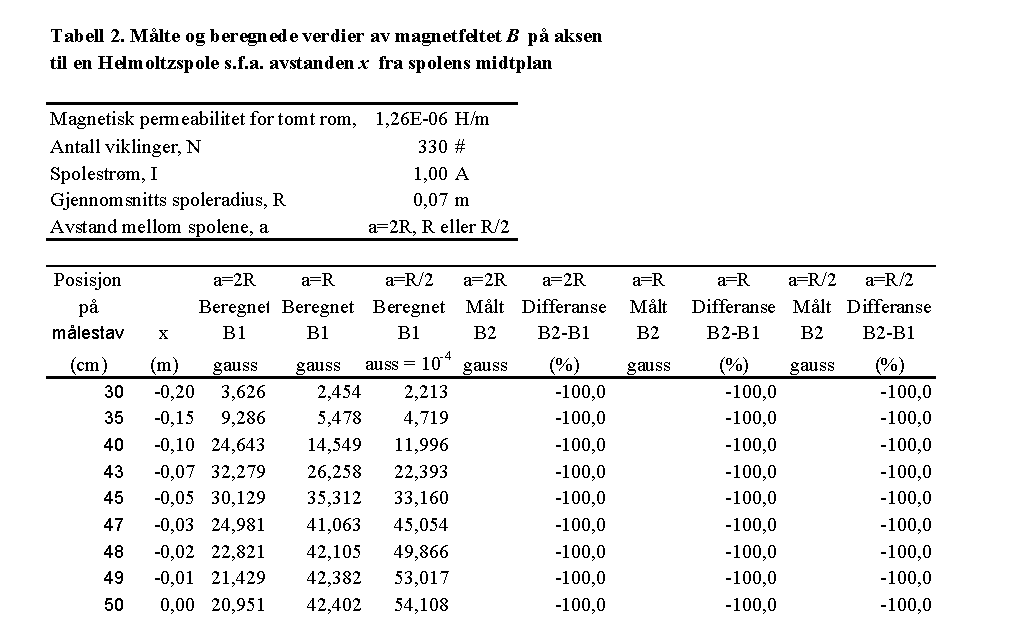
\includegraphics[width=0.8\textwidth]{fig/magnetfelt-tab2.eps}
%     \end{center}
%     \caption{%
%         Utdrag fra tabell for magnetfelt på aksen til Helmholtzspoler.
%     }
%     \label{magnetfelt.tab2}
% \end{figure}

\emph{4B. Present the result in a curve diagram}

The spreadsheet shall also be used for the calculation of expected magnetic field strengths as a result of Biot-Savart's law \eqref{eq:Biot.Savart3} and subsequent comparison with experimentally measured magnetic field strengths in section \ref{ch.magnetfelt.eksperimentelt}.

\emph{4C. Include a column for measured value of $B$ and a column for deviations between measured and calculated value given in \si{\percent} for $a = 2R$. Repeat this for the other two values   of $a$. Prepare to display the deviation graphically.} (A suggestion is given in the table in Table \ref{tab:example-table2}.)

Calculate also one of the values of $B$ by hand, and verify the value of the difference between calculated and measured.

\subsection{Anti-Helmholtz Coil}
%%%%%%%%%%%%%%%%
%%%%%%%%%%%%%%%%%%%%%%%%%%%%%%%%%%%%%% 
Anti-Helmholtz coils consist of two identical, short coils connected in series set up concentrically at a distance $a$ as shown in Figure \ref{magnetfelt.fig2a}, with opposite directions of the magnetic field. How do you find the field in this configuration?

\begin{marginfigure}
    \setlength{\unitlength}{0.6mm}
    \begin{picture}(120,80)(30,0)
        \linethickness{0.5mm}
        \put(44,79){\makebox(0,0)[b]{\large$\bigodot$}}
        \put(44,19){\makebox(0,0)[b]{\large$\bigoplus$}}
        \put(40,19){\framebox(8,8)}%[20,20]{KRN}
        \put(40,79){\framebox(8,8)}%[20,60]{KRN}
        \put(104,79){\makebox(0,0)[b]{\large$\bigoplus$}}
        \put(104,19){\makebox(0,0)[b]{\large$\bigodot$}}
        \put(100,19){\framebox(8,8)}%[20,20]{KRN}
        \put(100,79){\framebox(8,8)}%[20,60]{KRN}
        \put(74,47){\line(0,1){6}} 
        \put(30,50){\vector(1,0){100}} %x-axis
        %\qbezier(128, 51)(129, 50.5)(130,50)
        %\qbezier(128, 49)(129, 49.5)(130,50)
        \qbezier(126, 51.5)(128, 50.8)(130,50)
        \qbezier(126, 49)(128, 49.5)(130,50)
        %\color{magenta}
        \put(44,60){\line(1,0){60}} 
        \qbezier(47, 61)(47, 61)(44,60)
        \qbezier(47, 59)(47, 59)(44,60)
        \qbezier(102, 61)(102, 61)(104,60)
        \qbezier(102, 59)(102, 59)(104,60)
        %%\color{yellow}
        \thinlines
        \put(39.7,27.8){\framebox(8.4,51)}%[20,60]{KRN}
        \put(99.7,27.8){\framebox(8.4,51)}%[20,60]{KRN}
        \put(134,48){\makebox(0,0)[b]{\large$x$}}
        \put(74,62){\makebox(0,0)[b]{\large$a$}}
        \put(74,40){\makebox(0,0)[b]{\large O}}
        \put(26,64){\makebox(0,0)[b]{\large$R$}}
        \put(68,20){\makebox(0,0)[b]{\small\sf Windings}}
        \put(32,50){\vector(0,1){32}}
        %%\color{magenta}
        \put(55,22){\vector(-1,-0){5}} 
    \end{picture}
    \caption{%
Anti-Helmholtz coils consist of two identical, short coils connected in series set up concentrically at a distance $a$, with the current running opposite of each other.
\label{magnetfelt.fig2a}}
\end{marginfigure}

\emph{5A. Make a table of the magnetic flux density $B(x)$ on the axis of the Anti-Helmholtz coil in the area $\SI{-20}{\cm} < x < \SI{20}{\cm}$ for each of the three different distances $a = R/2, R$ and $2R$.}

\emph{5B. Present the result in a graph.}

The spreadsheet shall also be used for the calculation of expected magnetic field strengths as a result of Biot-Savart's law \eqref{eq:Biot.Savart3} and subsequent comparison with experimentally measured magnetic field strengths in section \ref{ch.magnetfelt.eksperimentelt}.

\emph{5C. Include a column for measured values   of $B$ and a column for discrepancies between measured and calculated values   given in \si{\percent} for $a = 2R$. Repeat this for the other two values   of $a$. Prepare the spreadsheet to display the deviation graphically.} (A suggestion is given in Table \ref{tab:example-table2}.)

Make a control calculation by hand of one of the calculated $B$. Check the calculated difference by entering the hand-calculated value.

\subsection{Solenoid \label{ch.magnetfelt.solenoide}}
%%%%%%%%%%%%%%%%%%%%%%%%%%%%%%%%%%%%%%%%%%%%%%%%%%%%%%%%%

The magnetic field at a point P on the axis of a solenoid can be found from Biot-Savart's law, and the result is
\begin{equation}
    B = \frac{N \mu_0 I} {2 \ell} \qty(\cos\theta_1 - \cos\theta_2),
    \label{eq:solenoide}
\end{equation}
where $\ell$ is the length of the solenoid and the angles $\theta_1$ and $\theta_2$ are defined in Figure \ref{magnetfelt.fig3}, and in a larger version in Figure \ref{magnetfelt.fig3_large}.
%
\begin{marginfigure}
\centering
    \setlength{\unitlength}{0.7mm}
    \rotatebox{90}{
    \begin{picture}(120,80)(30,30)
        %\linethickness{0.5mm}
        \newsavebox{\OneTurn}
        \savebox{\OneTurn}{
        \put(44,80){\makebox(0,0)[b]{\large$\bigodot$}}
        \put(44,20){\makebox(0,0)[b]{\large$\bigotimes$}}
        }
        \multiput(0,20)(5.1,0){20}{\usebox{\OneTurn}}
        \put(44,72){\line(1,0){120}} 
        \put(44,72){\line(0,1){2}} %origin up
        \put(44,72){\line(0,-1){2}}%origin down
        %\put(104,72){\line(0,-1){2}}
        \put(104,64){\makebox(0,0)[b]{\large{P}}} 
        \put(44,64){\makebox(0,0)[b]{\large{O}}}  
        %\color{red}
        \qbezier(44, 102.5)(103, 72)(103,72)
        \qbezier(79.5, 102.5)(103, 72)(103,72)
        \qbezier(141, 102.5)(103, 72)(103, 72)
        %\color{black}
        \multiput(77,42)(0,3.4){18}{\line(0,1){2}}
        \multiput(81,42)(0,3.4){18}{\line(0,1){2}}
        \put(143,72){\vector(0,1){30}}%locating R
        \put(143,102){\vector(0,-1){30}}%locating R
        \put(146,88){\makebox(0,0)[b]{\large$R$}}
        \put(79,106){\makebox(0,0)[b]{\large$\rightarrow$}}
        \put(79,106){\makebox(0,0)[b]{\large$\leftarrow$}}
        \put(79,110){\makebox(0,0)[b]{$\dd{x}$}}
        \put(104,70){\vector(-1,0){25}}%locating x
        \put(79,70){\vector(1,0){25}}%locating x
        \put(90,66){\makebox(0,0)[b]{\large$x$}} 
        \qbezier(68, 72)(65, 80)(70,88)
        \put(64,80){\makebox(0,0)[b]{\large$\theta_1$}} 
        \qbezier(90, 72)(90, 77)(96,81)
        \put(90,80){\makebox(0,0)[b]{\large$\theta$}} 
        \qbezier(94, 72)(102, 82)(112,80)
        \put(104,82){\makebox(0,0)[b]{\large$\theta_2$}} 
        
        \put(44,52){\line(0,1){2}} %origin up
        \put(44,52){\line(0,-1){2}}%origin down
        \color{black}
        \put(44,52){\line(1,0){57}}
        \put(101,50.6){\makebox(0,0)[b]{\large$\succ$}}
        \put(90,54){\makebox(0,0)[b]{\large$z$}} 
        \put(44,30.4){\line(1,0){95.5}}
        %\color{magenta}
        \put(44.8,29){\makebox(0,0)[b]{\large$\prec$}}
        \put(138,29){\makebox(0,0)[b]{\large$\succ$}}
        %\put(44,101.6){\line(1,0){95.5}}
        \put(90,24){\makebox(0,0)[b]{\large$\ell$}} 
    \end{picture}}
    \caption{%
        A solenoid. The angles are used for calculation of the magnetic field along the axis of the solenoid.
        See the main text for details.
        See Figure \ref{magnetfelt.fig3_large} for a larger version.
    }
    \label{magnetfelt.fig3}
\end{marginfigure}
%
Analytically the angles are given by
\begin{equation}
    \cos \theta_1 = \frac{z}{\sqrt{z^2 + R^2}}, \qquad
    \cos \theta_2 = - \frac{\ell - z}{\sqrt{(\ell - z)^2 + R^2}},
\end{equation}
where $R$ is the inner radius of the solenoid and $z$ is the distance from the left end of the solenoid to the point $P$. Inside the solenoid the angles are restricted to $\theta_1 \in \langle 0, \pi/2 \rangle$ and $\theta_2 \in \langle \pi/2, \pi \rangle$. The formula also applies outside the solenoid.
%

\begin{proof}
  \emph{We offer here a short proof of Equation \eqref{eq:solenoide}:} In equation \eqref{eq:Biot.Savart3} we have found magnetic fields on the axis at a distance $x$ from a single loop. In a solenoid we have many loops close together, we define current per unit length as $\flatfrac{I N}{\ell} = I n$, where $n$ is the number of windings per length. Flux density at a point P on the axis then receives a contribution from the thin current loop $\dd{I} = I n \dd{x}$ in position $x$, and according to the first part of equation \eqref{eq:Biot.Savart3} the flux density is 
  \begin{equation}
    \dd B 
    = \frac{\mu_0 \dd{I}}{4 \pi} \frac{2\pi R^2}{\qty(x^2 + R^2)^{3/2}}
    = \frac{\mu_0 I n}{2}  \frac{R^2}{ \qty( R^2 + x^2)^{3/2}} \dd{x} .
    \label{eq:solenoide2}
  \end{equation}
  % 
  With $\theta$ as the angle at point P between the solenoid axis and the periphery at position $x$ (Figure \ref{magnetfelt.fig3}) we see that $\tan \theta = R / x$, and differentiation of $x = R / \tan \theta$ gives
  \begin{equation}
    \dd{x} 
    = R \frac{-1}{\tan^2 \theta} \frac{1}{\cos^2\theta} \dd{\theta} 
    = -R \frac{1}{\sin^2\theta} \dd{\theta} .
  \end{equation}
  % 
  We notice that
  \begin{equation}
    \sin^3 \theta = \frac{R^3}{(R^2 + x^2)^{3/2}},
  \end{equation}
  so that
  \begin{equation}
    \dd{x} 
    = -R \frac{1}{\sin^3\theta} \sin\theta \dd{\theta}
    = -R \frac{(R^2 + x^2)^{3/2}}{R^3} \sin\theta \dd{\theta}
  \end{equation}
  and by substituting $\tan \theta = R / x$ in equation \eqref{eq:solenoide2} and inserting boundaries $\theta_2$ (right end, lowest $x$) to $\theta_1$ (left end, highest $x$), we will get
  % 
  \begin{equation}
    B(x) 
    = -\frac{\mu_0 I n}{2} \int_{\theta_2}^{\theta_1} \sin \theta \dd{\theta}
    = \frac{\mu_0 I n}{2} (\cos \theta_1 - \cos \theta_2),
    \label{eq:solenoide3}
  \end{equation}
  the result we wanted to show.
\end{proof}
% Formelen gjelder også utenfor solenoiden med $\theta_1 > \pi/2$ utenfor høyre ende og $\theta_2 < \pi/2$ utenfor venstre ende

\emph{5. What is the expression of the magnetic field deep inside the solenoid, and what is it at the end of the solenoid?}
\\
TIP: What are $\theta_1$ and $\theta_2$ at these positions?

Suppose you have a solenoid with $N = \SI{397}{\windings}$, $\ell = \SI{420}{\mm}$, $R = \SI{50}{\mm}$ and current $I = \SI{1.00}{\ampere}$.

\emph{6A. Make a table of the magnetic flux density $B(z)$ on the axis of the solenoid in the area $\SI{-10}{\cm} < z < \SI{50}{\cm}$ where $z = 0$ at the left edge of the solenoid.} % siunitx klarer ikke å merke tekstfamilien her...

%Hvis  $R \ll \ell$ og $x \neq 0$ og $x \neq \ell$ kan du ved rekkeutvikling finne at 
% Tatt ut denne approksimasjonen, da den ikke er god ved endene.
% Beregn forholdet B(X)/l på aksen -l \ t solenoiden i området2S:<J < x <s'o mm og framstill resultatet i et kurvediagram 

A suggested table is shown in Table \ref{tab:example-table3}.

\begin{table}[h]
  \centering
  \caption{Calculated and measured values of the magnetic field $B$ along the axis of a solenoid as a function of the distance $z$.\label{tab:example-table3}}
  \scriptsize
  \begin{tabular}{lrl}
    \hline
    Magnetic permeability for vacuum, $\mu_0$ & 1.26E-0.6 & H/m\\
    Number of windings, $N$ & 397 & \#\\
    Current, $I$ & 1.00 & A\\
    Inner loop radius, $R$ & 0.05 & m\\
    Length, $l$ & 0.42 & m\\
    \hline
  \end{tabular}
  
  \vspace{1em}
  \begin{tabular}{rrrrrrr}
    \hline
    Position & $z$ & $\cos \theta_1$ & $\cos \theta _2$ & Calculated & Measured & Difference\\
    (cm) & (m) & & & (gauss) & (gauss) & (\%)\\
    \hline
60 & -0.10 & -0.894 & -0.995 & 0.600 &  & -100.0\\
55 & -0.05 & -0.707 & -0.994 & 1.707 &  & -100.0\\
53 & -0.03 & -0.514 & -0.994 & 2.848 &  & -100.0\\
52 & -0.02 & -0.371 & -0.994 & 3.696 &  & -100.0\\
51 & -0.01 & -0.196 & -0.993 & 4.736 &  & -100.0\\
50 & 0.00 & 0.000 & -0.993 & 5.899 &  & -100.0\\
49 & 0.01 & 0.196 & -0.993 & 7.062 &  & -100.0\\
  \end{tabular}
\end{table}
%
% BEGIN RECEIVE ORGTBL magnetfelt.tab3
\begin{tabular}{rrrrrlr}
% 60 & -0.10 & -0.894 & -0.995 & 0.600 &  & -100.0\\
% 55 & -0.05 & -0.707 & -0.994 & 1.707 &  & -100.0\\
% 53 & -0.03 & -0.514 & -0.994 & 2.848 &  & -100.0\\
% 52 & -0.02 & -0.371 & -0.994 & 3.696 &  & -100.0\\
% 51 & -0.01 & -0.196 & -0.993 & 4.736 &  & -100.0\\
% 50 & 0.00 & 0.000 & -0.993 & 5.899 &  & -100.0\\
% 49 & 0.01 & 0.196 & -0.993 & 7.062 &  & -100.0\\
\end{tabular}
% END RECEIVE ORGTBL magnetfelt.tab3
\begin{comment}
#+ORGTBL: SEND magnetfelt.tab3 orgtbl-to-latex :splice nil :skip 0
| 60 | -0.10 | -0.894 | -0.995 | 0.600 |   | -100.0 |
| 55 | -0.05 | -0.707 | -0.994 | 1.707 |   | -100.0 |
| 53 | -0.03 | -0.514 | -0.994 | 2.848 |   | -100.0 |
| 52 | -0.02 | -0.371 | -0.994 | 3.696 |   | -100.0 |
| 51 | -0.01 | -0.196 | -0.993 | 4.736 |   | -100.0 |
| 50 |  0.00 |  0.000 | -0.993 | 5.899 |   | -100.0 |
| 49 |  0.01 |  0.196 | -0.993 | 7.062 |   | -100.0 |
\end{comment}

\emph{6B. Present the result in a line diagram}

The spreadsheet shall also be used for the calculation of expected magnetic field strengths as a result of Biot-Savart's law \eqref{eq:Biot.Savart3} and subsequent comparison with experimentally measured magnetic field strengths in section \ref{ch.magnetfelt.eksperimentelt}.

\emph{6C. Include a column for measured value of $B$ and a column for deviations between measured and calculated value given in \si{\percent}}. (A suggestion is given in the table in Table \ref{tab:example-table3}.)

\begin{figure*}[bp]
\centering
    \setlength{\unitlength}{1.3mm}
    \begin{picture}(120,80)(30,20)
        %\linethickness{0.5mm}
        \savebox{\OneTurn}{
        \put(44,80){\makebox(0,0)[b]{\large$\bigodot$}}
        \put(44,20){\makebox(0,0)[b]{\large$\bigotimes$}}
        }
        \multiput(0,20)(5.1,0){20}{\usebox{\OneTurn}}
        \put(44,72){\line(1,0){120}} 
        \put(44,72){\line(0,1){2}} %origin up
        \put(44,72){\line(0,-1){2}}%origin down
        %\put(104,72){\line(0,-1){2}}
        \put(104,64){\makebox(0,0)[b]{\large{P}}} 
        \put(44,64){\makebox(0,0)[b]{\large{O}}}  
        %\color{red}
        \qbezier(44, 102.5)(103, 72)(103,72)
        \qbezier(79.5, 102.5)(103, 72)(103,72)
        \qbezier(141, 102.5)(103, 72)(103, 72)
        %\color{black}
        \multiput(77,42)(0,3.4){18}{\line(0,1){2}}
        \multiput(81,42)(0,3.4){18}{\line(0,1){2}}
        \put(143,72){\vector(0,1){30}}%locating R
        \put(143,102){\vector(0,-1){30}}%locating R
        \put(146,88){\makebox(0,0)[b]{\large$R$}}
        \put(79,106){\makebox(0,0)[b]{\large$\rightarrow$}}
        \put(79,106){\makebox(0,0)[b]{\large$\leftarrow$}}
        \put(79,110){\makebox(0,0)[b]{$\dd{x}$}}
        \put(104,70){\vector(-1,0){25}}%locating x
        \put(79,70){\vector(1,0){25}}%locating x
        \put(90,66){\makebox(0,0)[b]{\large$x$}} 
        \qbezier(68, 72)(65, 80)(70,88)
        \put(64,80){\makebox(0,0)[b]{\large$\theta_1$}} 
        \qbezier(90, 72)(90, 77)(96,81)
        \put(90,80){\makebox(0,0)[b]{\large$\theta$}} 
        \qbezier(94, 72)(102, 82)(112,80)
        \put(104,82){\makebox(0,0)[b]{\large$\theta_2$}} 
        
        \put(44,52){\line(0,1){2}} %origin up
        \put(44,52){\line(0,-1){2}}%origin down
        \color{black}
        \put(44,52){\line(1,0){57}}
        \put(101,50.6){\makebox(0,0)[b]{\large$\succ$}}
        \put(90,54){\makebox(0,0)[b]{\large$z$}} 
        \put(44,30.4){\line(1,0){95.5}}
        %\color{magenta}
        \put(44.8,29){\makebox(0,0)[b]{\large$\prec$}}
        \put(138,29){\makebox(0,0)[b]{\large$\succ$}}
        %\put(44,101.6){\line(1,0){95.5}}
        \put(90,24){\makebox(0,0)[b]{\large$\ell$}} 
    \end{picture}
    \caption{%
        A solenoid. The angles are used for calculation of the magnetic field along the axis of the solenoid.
        See the main text for details.
    \label{magnetfelt.fig3_large}
    }
\end{figure*}


\FloatBarrier % Fix solenoid figure floating 
\subsection{Python Data Analysis}
The previous tasks can be done in Python, for example. It is advisable to save the data in text files. Here we use comma separated files as shown in the margin.
\begin{marginlisting}
  % \caption{Example of CSV file.}
  Example of a CSV file.
\begin{verbatim}
# Position (m), B-field (Gauss)
0.245,0.0
0.295,0.623
...
\end{verbatim}
\end{marginlisting}
Here, the first column represents the \emph{Position}, and the second column represents \emph{Measured} in Table \ref{tab:example-table}. The remaining columns can be calculated in Python. To read the data, we create the following code:

\begin{lstlisting}[language=python]
# Assumes numpy imported as np.
def read_CSV(filename):
   data = np.loadtxt (filename, delimiter = ',')
   xe = data [:, 0]
   Be = data [:, 1]
   return xe, Be
\end{lstlisting}
In the function \texttt{read\_CSV}, the text file with filename \emph{filename} is read. The position data, located in the first column, is stored in the variable \texttt{xe} and the data for the measured magnetic field is stored in the variable \texttt{Be}.

The next thing we need to do is implement a function that calculates the magnetic field according to equation \eqref{eq:kort.spole}. We can do this as follows:

\begin{lstlisting}[language=python]
def B_field_short_coil(x):
    prefactor = N * mu_0 * I0 / (2 * R)
    return prefactor * (1.0 + (x / R) ** 2) ** (-1.5)
\end{lstlisting}
To plot the result for the calculated field, we add some lines in the \texttt{main} function. We also need to define some parameters used in the calculation. The whole program then looks like this:

\begin{marginlisting}[-3cm]
A quick note about the \texttt{main} function.
You will quite often see code with a function called \texttt{main}, and then a code
\begin{lstlisting}[language=python,style=kaolstplain,breaklines=false]
if(__name__=='__main__'):
    main ()
\end{lstlisting}
at the end of the file.
This is a common convention which is useful for larger projects using several files.
It makes it easier for others to see what is the ``entry point'' of your code, and also prevents accidental execution of code.
Feel free to search the web for this if you want to know more.
\end{marginlisting}
\begin{lstlisting}[language=python]
import numpy as np
from matplotlib import pyplot as plt

N = 330 # [] number of windings
I0 = 1.0 # [A] current
mu_0 = 4.0 * np.pi * 1e-7 # [H / m] permeability in empty space
R = 0.07 # [m] radius
x0 = 0.400 # [m] center of coil

def B_field_short_coil (x):
    prefactor = N * mu_0 * I0 / (2 * R)
    return prefactor * (1.0 + (x / R) ** 2) ** (- 1.5)

def read_CSV(filename):
   data = np.loadtxt (filename, delimiter = ',')
   xe = data [:, 0]
   Be = data [:, 1]
   return xe, Be
    
def main ():
    xe, Be = read_CSV("short_spool.csv")
    
    # Calculate the B field
    xb = np.linspace (xe [0], xe [-1], 100) # multiple data points
    Bb = B_field_short_coil (xb) * 1e4 # calculated B-field (Gauss)
    
    # Plot the results
    plt.plot (xb, Bb, label = 'Calculated')
    plt.plot (xe, Be, '.', label = 'Measurement data')
    plt.xlabel ('Distance from center of coil (m)')
    plt.ylabel ('Magnetic field (Gaussian)')
    plt.legend ()
    plt.show ()
    
if (__name__ == '__main__'):
    main ()
\end{lstlisting}

You can now create more functions to plot the results for a Helmholtz coil and a solenoid. Remember that it often pays to divide the program into smaller functions. This makes the code easier to read, but also allows you to reuse much of the code for other purposes.
More examples of plotting can be found at the NumFys webpage: \url{https://nbviewer.jupyter.org/urls/www.numfys.net/media/notebooks/basic_plotting.ipynb}.

\subsection{Hall effect probe}
%%%%%%%%%%%%%%%%%%%%%%%%%%%%%%%%

\begin{marginfigure}[-2cm]
    \setlength{\unitlength}{0.6mm}
    \begin{picture}(120,80)(40,20)
        \put(50,30){\framebox(40,10)}%lower rectangle
        \put(90,70){\dashbox{0.2}(40,10)}%upper rectangle
        %\qbezier(70, 55)(70,80)(120,100)
        %\qbezier(50, 30)(58,50)(66,70)
        \put(50,30){\line(1,1){40}}
        \put(50,40){\line(1,1){40}}
        \put(90,30){\line(1,1){40}}
        \put(90,40){\line(1,1){40}}
        \put(70,55){\tiny$\bullet$}%left side
        \multiput(70,55.5)(-2,0){2}{\line(-1,0){1}}
        \multiput(67,55.5)(0,2){2}{\line(0,1){1}}
        \put(67,57){\line(0,1){35}}
        \put(110,55){\tiny$\bullet$}%right side
        \put(110.5,55.5){\line(1,0){25}}
        %\color{green}
        \put(136,55.5){\line(0,1){36.5}}
        \put(136,55.5){\line(0,1){36.5}}
        %\put(136,55.5){\line(0,1){36.5}}
        %\put(67,92){\line(1,0){75}}
        \put(67,92){\line(1,0){28}}
        \put(95,91.5){\tiny$\bullet$}     %left top
        \put(99,91.5){\large$V_\text{H}$} 
        \put(108,91.5){\tiny$\bullet$}    %right top
        %\color{red}
        \put(136,92){\line(-1,0){28}}
        \put(69.5,35){\tiny$\bullet$}%front
        \put(109.5,75){\tiny$\bullet$}%back
        %\put(70,35){\line(1,1){60}}
        \put(60,25){\line(1,1){10}}    %Current in
        \put(55,20){\Huge\vector(1,1){6}}   %Current in arrow
        \put(110,75){\vector(1,1){12}} %Current out
        \put(90,56){\vector(1,0){10}}
        \put(90,56){\vector(-1,-1){7}}
        \put(95,50){\footnotesize$\va*{F}$}
        \put(80,45){\footnotesize$\va*{v}$}
        \put(96,63){$\va*{B}$}
        \put(85,55){\footnotesize$q$}
        \put(89.25,55.25){\tiny$\bullet$}
        \put(95,58){\vector(0,1){9}}
        \put(96,63){$\va*{B}$}
        \put(43,32){\Huge$\updownarrow$}
        \put(40,33){\large$d$}
        \put(60,20){\large$I$}
        \put(49,24.5){\Huge$\longleftarrow$}
        \put(68,25){\large$b$}
        \put(73,24.5){\Huge$\longrightarrow$}
    \end{picture}
    % \caption{Halleffekt i en halvlederprobe. Strøm $I$ påtrykkes mellom de to minste endevegger.}
    \caption{Hall effect in a semiconductor probe. A current $I$ is made to flow thorugh the sample, causing the electrons to experience a force $\vec{F}$.}
    \label{magnetfelt.fig4}
\end{marginfigure}
When electrons move at speed $\va*{v}$ in a semiconductor located in a magnetic field $\va*{B}$ as shown in Figure \ref{magnetfelt.fig4}, the electrons will bend to one side. The deflection is given by the Lorentz force $\va*{F} = q(\va*{v} \cross \va*{B})$, where $q = -e$ for electrons.

%\begin{figure}[h]
%\begin{center}
%%\vspace{25mm}
%\includegraphics[width=90mm]{fig/magnetfelt.fig4.eps}
%\end{center}
%\caption{\sf Halleffekt i en halvlederprobe. Strøm $I$ påtrykkes mellom de to minste endevegger.}
%\label{magnetfelt.fig4}
%\end{figure}

The Lorentz force acts normal to the current direction and normal to $B$; the deflection due to this causes the electron concentration to become stronger against one wall of the semiconductor. An electric field $\va*{E}$ thus builds up in the conductor with the same direction as the Lorentz force, and this field gives an additional force $\va*{F} = q \va*{E}$ on the electrons. Equilibrium will quickly arise where electrostatic force and Lorentz force are equal so that
\begin{equation}
    \va*{F} =  q \va*{E} + q(\va*{v} \cross \va*{B}) = \va*{0}
    \quad \Rightarrow \quad
    \va*{E} = -\va*{v} \cross \va*{B} .
\end{equation}

The speed $v$ of the electrons through the semiconductor is determined by the current at the expression $I = nqvA$, where $n$ is the density of electrons and $A = bd$ is the cross section in the conducting direction, see Figure \ref{magnetfelt.fig4}. This gives
\begin{equation}
    v = \frac{I}{A} \frac{1}{nq} 
        = \frac{I}{bd} R_\text{H},
\end{equation}
where we have defined the Hall constant $R_\text{H} = 1/nq$.

With $b$ equal to the width of the probe, the voltage $V_\text{H} = E b$ will form across the side walls. If we disregard the sign and use that $\va*{v} \perp \va*{B}$ we get the Hall voltage $V_\text{H}$:

\begin{equation}
    V_\text{H} = Eb
        =  vBb 
        = \frac{R_\text{H} I}{d} B,
    \label{eq:Hall}
\end{equation}

where $d$ is the thickness of the Hall probe where the magnetic field $B$ is present. The hall constants $R_\text{H}$ and $d$ are constants for a given probe and the current $I$ is kept constant. The magnetic flux density $B$ normal to the probe will then be proportional to the Hall voltage $V_\text{H}$ which is measured with a voltmeter.

%\vspace{1cm}
\begin{marginfigure}
    % \begin{minipage}[b]{\linewidth}
    % \centering
    \begin{overpic}[scale=0.5]{fig/HallAx.eps}
        % \put(-12, 14){\large$1$}
        \put(115,14){\large$\va*{B}$}
        \put(95,14){\Huge$\rightarrow$}
        \label{fig:figure1}
    \end{overpic}
    % \end{minipage}%
    %
    % \begin{minipage}[b]{\linewidth}
    % \centering
    \begin{overpic}[scale=0.5]{fig/HallTr.eps}
        % \put(-12, 14){\large$2$}
        \put(100, 14){\Huge$\downarrow$}
        \put(112, 14){\large$\va*{B}$}
    \end{overpic}
    \label{fig:figure2}
    % \end{minipage}
    \caption{%
        Probe geometries: \textbf{(Top)} Axial probe, \textbf{(Bottom)} Transversal probe.
    }
    \label{magnetfelt.fig8}
\end{marginfigure}

%%%%%\vspace{2cm}

The hall effect is used in for example magnetometers
\sidenote{Also known as Gaussmeters and Teslameters.}
, instruments for measuring magnetic fields. A Hall effect magnetometer will essentially consist of a current source that provides a constant current $I$ through a probe, and a voltmeter. The probe is placed in the magnetic field to be measured. Through a calibration process, the relationship between the measured Hall voltage and the magnetic field can be established and the voltage reading unit is graded directly in $\si{\tesla} = \si{\weber/\square\m}$ or $\si{gauss} = \SI{e-4}{\tesla}$.

In practice, the extent of a Hallprobe is of the order of a few \si{\square\mm}. Two different probe geometries are common: transverse probes and axial probes, as shown in Figure \ref{magnetfelt.fig8}.

Typical value for the electron density in a doped semiconductor is $n = \SI{e20}{\elektroner/\m\cubed}$. By comparison, copper has $n = \SI{e28}{\elektroner/\m\cubed}$. In our magnetometers we have $I = \SI{20}{\milli\ampere}$ and $d = \SI{1,0}{\mm}$. Assume that the magnetic field varies from 1 to \SI{100}{\gauss}.

\emph{7A. What measuring range must the magnetometer's voltmeter have to measure in this magnetic field range? (Assume at $n = \SI{e20}{\elektroner/\m\cubed}$.)}
  
\emph{7B. Why do you think semiconductors are used in magnetic field probes? Explain why e.g. copper will not be a suitable material.}

\emph{7C. Also explain why an insulator will not be a suitable material in a magnetic field probe.}


\subsection{Magnetic scattering fields}

In the laboratory, there are background magnetic fields, or ``noise'', which can interfere with the magnetic field measurements.
These noise fields have three main sources:
\vspace{-4mm}
\begin{itemize}
    \item the Earth's magnetic field,
    \item magnetic fields from magnetic materials in building structures and fixtures,
    \item induced magnetic fields from for example \SI{230}{\volt} power cords.
\end{itemize}

The Earth's magnetic field, which is constant and of the order of magnitude \SI{1}{\gauss}, is believed to originate from convection currents of electric charges in the Earth's liquid core. Assume that in the middle of the Earth's interior there is a current loop perpendicular to the Earth's axis of rotation. Let the radius of the current loop be $R = R_\text{j}/4$, where $R_\text{j} = \SI{6371}{\km}$ is the radius of the Earth. The axial component of the magnetic field in position $x$ on the axis of such a current loop is given by equation \eqref{eq:Biot.Savart3}, which reads
\[
  B_x = \frac{\mu_0 I}{4 \pi} \frac{2\pi \xi^2}{\left( x^2 + \xi^2 \right)^{3/2}}
      = \frac{\mu_0 I}{2 \xi} \qty(1 + \frac{x^2}{\xi^2})^{-3/2}.
\]

\emph{8. How large must the current in the loop be for the magnetic field on the Earth's surface at the pole ($x = R_\text{j}$) to be equal to \SI{1}{\gauss}? }

%\emph{8B. Er det en god antakelse å bruke $\mu_0$ som permeabilitet i jordas indre? }

Contributions to the background magnetic field from the building and the inventory will depend on the building and construction materials used. You will evaluate the contributions to this in the laboratory through your own measurements.

Contribution to the background field from the currents in non-shielded wires can be estimated by calculating the field set up by a long straight conductor leading the current $I$. The azimuthal component of the magnetic field at a distance $r$ from a long conductor can be found from \sidenote{Derivation in e.g. Lillestøl et al. \cite[Ch.~23.5]{lillestol}.} Biot-Savarts Law \eqref{eq:Biot.Savart2}
\begin{equation}
    B_\theta (r) = \frac{\mu_0 I}{2\pi r} .
\end{equation}

\emph{9. How large is the magnetic flux density at a distance \SI{5}{\cm} from a long \SI{230}{\volt} mains lead due to a current \SI{1}{\ampere} in this wire?}

\subsection{Magnetic field-free room \label{ch.mymetall}}
%%%%%%%%%%%%%%%%%%%%%%%%%%%%%%%%%%%%%%%%%%%%%%%%%%%%%%%

The permanent magnetic field on the Earth's surface leads to problems with zeroing of magnetometers. However, magnetic fields can be shielded by using materials with high permeability. Pure iron can be used. There are also special alloys that have even higher permeability $\mu$ and thus shields even better. An example is mu-metal\sidenote{Mu-metal is an alloy of \SI{77}{\percent} nickel, \SI{15}{\percent} iron plus some copper and molybdenum. It got its name due to very high value for magnetic permeability, $\mu$.}. Magnetmometers are usually zeroed by inserting the probe into a chamber that shields it from the Earth's magnetic field during zeroing.

%\emph{10. Hvordan ville du utforme et kammer av mymetall, med et lite hull i enden, på en slik måte at det inne i kammeret ble fritt for magnetfelt? }
%\footnote{TIPS: Ta ved utformingen av kammeret hensyn til at magnetiske feltlinjer må alltid følge en sluttet bane.}

\section{Experimental \label{ch.magnetfelt.eksperimentelt}}
%%%%%%%%%%%%%%%%%%%%%%%%%%%%%%%%%%%%%%%%%%%%%%%%%%%%%%%%%%%%%%%%%%%%%%%%%%%%%%

%%%%%%%%%%%%%%%%%%%%%%%%%%%%%%%%%%%%%%%%%%%%%%%%%%%%%%%%%%%%%%%%%%%%%%%%%%%%%%
\subsection{Equipment}
%%%%%%%%%%%%%%%%%%%%%%%%%%%%%%%%%%%%%%%%%%%%%%%%%%%%%%%%%%%%%%%%%%%%%%%%%%%%%%

The experiment uses PASCO's data logging system (Capstone) with interfaces and sensors for magnetic fields and position.
The following instruments are included in the line-up:
\vspace{-4mm}
\begin{itemize}
    \item \textbf{Interface.} PASCO 550 Universal Interface.
    \item \textbf{Magnetic field sensor.} PASCO Magnetic Field Sensor CI-6520A. \ \
    Measuring range: \SI{0,01}{\G} - \SI{100}{\kilo\G}. \ \
    Resolution: \SI{50}{\milli\G}.
    Accuracy: 10 \% of reading
    \item \textbf{Zero field chamber.} PASCO Zero Gauss Chamber EM-8652.
    \item \textbf{Position sensor.} PASCO Rotary Motion Sensor PS-2120A. Catalog \ \
    Resolution: \SI{0,09}{\degree}. \ \
    Radii on the three pulleys: \SI{10}{\mm}, \SI{29}{\mm}, \SI{48}{\mm}.
    \item \textbf{Short coils.} 330 Vikings, 22 Vikings / Team $\cross$ 15 Teams \ \
    Inner diameter \SI{126}{\mm}, Outer diameter \SI{154}{\mm}. \ \
    Wire: lacquer-insulated copper, diameter \SI{0,75}{\mm}, maximum coil current: \SI{1,0}{\ampere}.
    \item \textbf{Solenoid.} 368 windings, length $\sim \SI{400}{\mm}$, inner diameter \SI{100}{\mm}. \ \
    Wire: lacquer-insulated copper, diameter \SI{1,0}{\mm}, maximum solenoid current \SI{1,0}{\ampere}.
    \item \textbf{Multimeter.} Escort Mod. EDM 168A, or equivalent.
    %\item \textbf{Datamaskin} med printer.
    \item \textbf{Miscellaneous:} Meter, screwdriver.
    \item \textbf{Power supply.} Mascot Type 719. Range: 0- \SI{30}{\volt}, \SI{30}{\milli\ampere} - \SI{2}{\ampere}. \label{magnetfelt.kraftforsyning}
    %\\[1mm]
    This is a combined power-controlled / voltage-controlled power supply. That is, \ it can supply a constant current or a constant voltage, up to a certain maximum load. The box has two adjustment buttons, one for voltage marked "$0 \rightarrow \SI{30}{\volt}$" and one for current marked "$\SI{30}{\milli\ampere} \rightarrow \SI{2}{\ampere}$".
    \begin{description}
      \item[Current controlled power supply (current source)] the voltage adjustment is set to maximum. The current is regulated with the current adjustment knob.
      \item[Voltage controlled power supply(voltage source)]  the power adjustment is set to maximum. The voltage is regulated with the voltage adjustment knob.
    \end{description}
    When current controlled, the maximum current that may be supplied is \SI{2}{\ampere}, given that the  resistance is maximum $R = U/I = \SI{30}{\volt} / \SI{2}{\ampere} = \SI{15}{\ohm}$.
    The box also has a button marked ``range'' which can limit the maximum voltage to \SI{15}{\volt} instead of the standard \SI{30}{\volt}. If \SI{15}{\volt} is selected, the maximum output resistance will be $R = U/I = \SI{15}{\volt} / \SI{2,0}{\ampere} = \SI{7,5}{\ohm}$. At higher output resistance, the output voltage will be kept at maximum value and the current will be lower.\\

    There is a corresponding maximum regulation for voltage-controlled power supply. \SI{30}{\volt} maximum voltage can be given to a resistance of $R = U/I = \SI{30}{\volt} / \SI{2,0}{\ampere} = \SI{15}{\ohm}$. At lower resistance, the supply will not be able to provide enough current so that the voltage will drop.
\end{itemize}

\subsection{Calibration of the Hall probe}
%%%%%%%%%%%%%%%%%%%%%%%%%%%%%%%%%%%%%

It is difficult to produce Hall probes with exactly the same Hall constants. The Hall voltage that occurs at a given magnetic field and current may therefore vary slightly from probe to probe. In order to be able to use several probes for the same Gaussmeter, each probe has often assigned a calibration number which is used to adjust the gain of the Gaussmeter's voltmeter so that the meter shows the correct magnetic field. PASCO's sensors are adjusted and a calibration is not normally needed. Before use, the sensor must be reset.

\textbf{Resetting:}
\vspace{-4mm}
\begin{itemize}
    \item Set the area knob on the sensor to position 1x and axial.
    \item Insert the probe into the zero field chamber and press the zero adjustment button.
%\item Gjenta prosedyren hvis område endres.
%\item Sett områdeknappen i stilling 1 K.
\end{itemize}

%\textbf{MERK:} Før gaussmeteret er klart til bruk må det varmes opp i 15--20 min. Under oppvarmingen vil kalibreringen og nullstillingen drive. Før du begynner å ta nøyaktige målinger må du derfor gjenta kalibrering og nullstilling. \\
\textbf{Note:} When changing the measuring range, make a new reset!

\textbf{Units and signs of the Hall probe:}
\vspace{-4mm}
\begin{itemize}
    \item The meter shows the magnetic flux density, $B$, of the device you select in Capstone.
    \item The Gaussian meter shows \emph{positive} signs when the field lines have direction \emph{into} the cylindrical tip of the probe.
\end{itemize}

\subsection{Magnetic scattering fields}
%%%%%%%%%%%%%%%%%%%%%%%%%%%%%%%%%%%%%

Task:
\emph{Investigate the magnetic background fields, noise fields, in the laboratory.}
% \vspace{-5mm}
\begin{itemize}
\item How does the measured direction of the earth's magnetism correspond to the assumed direction of our latitude?
  \sidenote{The magnetic north pole is located near the geographical south pole. Magnetic field lines are closed curves and have direction from magnetic north pole to south pole outside of the magnet and from south pole to north pole inside the magnet.}
    \item Compare the results with results from the other groups. Is there variation of the measured earth magnetism within the laboratory?
    \item Will the magnetic field from the iron in the laboratory tables be able to interfere with the measurements?
\end{itemize}

%Som allerede nevnt er det strøfelt fra jordmagnetismen, elektriske ledninger, jernholdige materialer som laboratoriebenker etc.}

%Du bør sette gaussmeteret i stilling 10x for disse målingene (og husk å nullstille på ny!)

\subsection{Statistical error in measurements}
%%%%%%%%%%%%%%%%%%%%%%%%%%%%%%%%%%%%%

Reading magnetic field strengths from the Hall probe will give a somewhat varying result. You can use this to find the statistical error.

Task:
\emph{Investigate statistical errors in the measurements:}
\begin{itemize}
    \item Connect the sensors in the PASCO interface and the computer interface. Start Capstone and get ready for data sampling.
    \item Reset and sample data in \SI{10}{\s}. Select data and perform a statistical analysis with built-in functionality in Capstone. What is the standard deviation of the data? What standard deviations do you get if you sample in \SI{1}{\s} and \SI{100}{\s}? How many samples should you use?
    \item Use the standard deviation as an error in your data from the Hall probe.
\end{itemize}

\subsection{Magnetic field in short coil}
%%%%%%%%%%%%%%%%%%%%%%%%%%%%%%%%%%%%%

Task:
\emph{Investigate the magnetic field along the central axis of a short coil.}
 
%Drøfting av måleprosedyren: 

To measure the magnetic field, you can either hold the coil and move the Hall probe or you can attach the Hall probe and move the coil.
Which of these is best to use? Motivate your answer!
%I våre eksperimenter er siste løsning den beste fordi vi da unngår korrigering av gaussmeteravlesningene pga. det varierende strøfeltet langs spoleaksen. Når Hallproben sitter fast vil strøfeltet rundt proben være konstant og kan nulles ut vha. gaussmeterets nullstilling og feltet fra spolen kan følgelig leses direkte. 

\textbf{Procedure:}
\begin{itemize}
    \item Mount the rotation sensor on the stand.
    \item Connect the sensors to the interface and the interface of the computer. Start Capstone and get ready for data sampling.
    \item Mount a short spool on the movable carriage.
    \item Adjust the position of the magnetic field sensor so that it is on the coil axis. Use a bubble level.
    %\item Klargjør kraftforsyningen. 
    %Sjekk at den er avslått og justeringsknappene for strøm og spenning er skrudd helt ned.
    %Innstill til strømstyrt kraftkilde (se beskrivelsen av kraftforsyning side \pageref{magnetfelt.kraftforsyning}). 
    %\item Klargjør multimeteret.\\
    %Sjekk at det er avslått, sett AC/DC innstillingen i stilling DC og funksjonsvelgeren for strømmåling i området 0 - 20 A.\\
    %VIKTIG: Bruk kontakten for tilkopling av likestrøm i området 0 - 20 A. %Bruk denne, ellers går mulitmeterets sikring umiddelbart.
    \item Connect the coil circuit as shown in Figure \ref{magnetfelt.fig6}. \ \
    IMPORTANT: The power supply must be switched off during connection. Select current measurement on both the power supply and the multimeter. Use the 10A input on the multimeter.\\
    - Ask the lab supervisor to approve the connection.
    \item Reset the magnetic field sensor. (It is safest to break the coil circuit during zeroing.)
      \begin{marginfigure}[-10cm]
        \centering
        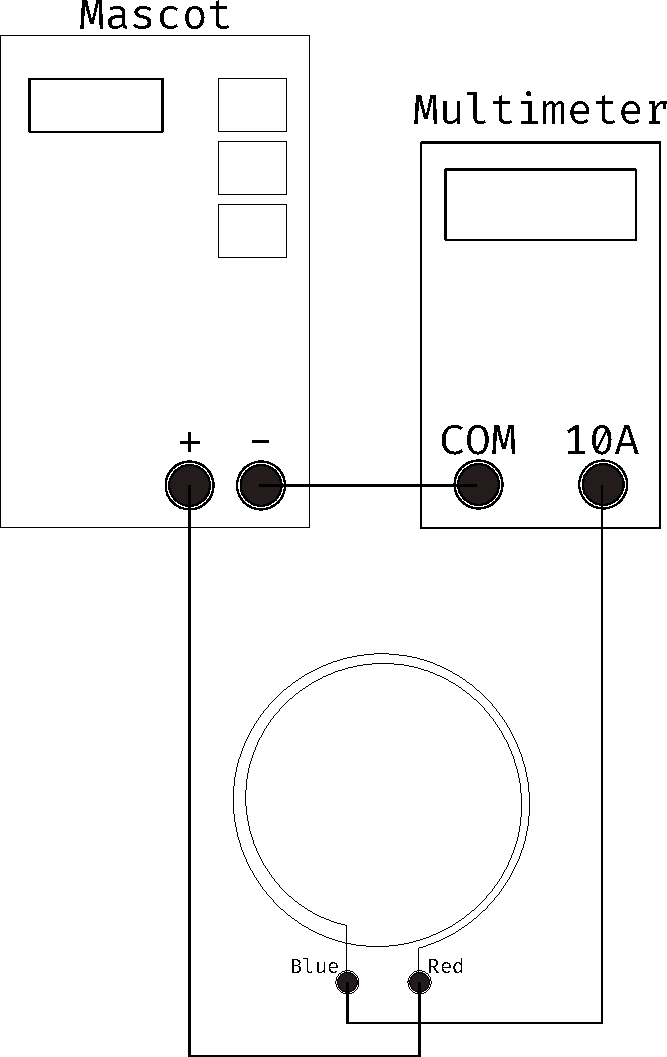
\includegraphics[width=0.8\textwidth]{fig/circuit_single_coil}
        % \vspace{-4cm}
        % \setlength{\unitlength}{0.6mm}
        % \begin{picture}(120,20)(20,0)
        %     \put(30,5){\line(1,0){88}}
        %     \put(118,5){\line(0,1){23}}
        %     \put(30,5){\line(0,1){14}}
        %     \qbezier(118, 28)(124, 28)(129,35)
        %     \qbezier(129, 35)(132, 40)(132,45)
        %     \qbezier(132,45)(132, 52)(125,58)
        %     \qbezier(125,58)(117, 63)(108,58)
        %     \qbezier(108,58)(102, 54)(101,45)
        %     \qbezier(101,45)(101, 38)(105,34.5)
        %     \qbezier(105,34.5)(109, 30)(115,30)
        %     %\color{red}
        %     \qbezier(115,30)(126, 31)(129,40)
        %     \qbezier(129,40)(132, 55)(118,58)
        %     \qbezier(118,58)(105, 59)(103,45)
        %     \qbezier(103,45)(102, 35)(114,32)
        %     \put(120,10){\Large$\uparrow$}%
        %     \put(125,10){\large$I$}%
            
        %     \put(50,15){\framebox(15,25)}%Multimeter
        %     \put(52.5,32){\framebox(10,5)}%Multimeter display
        %     \put(56,20){\circle{3}}%
        %     \put(55,18.7){\small$\bullet$}%
        %     \put(62,20){\circle{3}}%
        %     \put(60.7,18.7){\small$\bullet$}%
            
        %     \put(61.5,20){\line(1,0){53}}
        %     \put(114,32){\line(0,-1){12}}
        %     \put(52,16){\tiny\sf COM}%
        %     \put(60,16){\tiny\sf 10A}% 
        %     \put(45,45){\sf Multimeter}%
        %     %\color{red}
        %     \put(114,20){\circle{3}}%
        %     \put(113,18.7){\small$\bullet$}%
        %     \put(118,20){\circle{3}}%
        %     \put(116.7,18.7){\small$\bullet$}%
        %     \put(100,22){\sf Blue}%
        %     \put(119,22){\sf Red}%
        %     %\color{green}
        %     %%%%%%%%%Mascot begins
        %     \put(20,15){\framebox(20,34)}%Mascot
        %     \put(22,40){\framebox(9,5)}%Mascot
        %     \put(35,43){\framebox(3,5)}%Mascot
        %     \put(35,36){\framebox(3,5)}%Mascot
        %     \put(35,29){\framebox(3,5)}%Mascot
        %     \put(30,20){\circle{3}}%
        %     \put(28.8,18.7){\small$\bullet$}%
        %     \put(36,20){\circle{3}}%
        %     \put(34.6,18.7){\small$\bullet$}%
        %     \put(28,23){$+$}%
        %     \put(34,23){$-$}%
        %     \put(35,20){\line(1,0){22}}%Mascot-to-Multimeter
        %     \put(23,54){\sf Mascot}%
        %     %%%%%%%%%Mascit ends
        %     %\put(90,70){\dashbox{0.2}(40,10)}%upper rectangle
        % \end{picture}
        \caption{%
            The coil circuit.
            Mascot power supply, multimeter, and the coil are shown.
            Note the direction of the windings, and where the coil is here shown from the direction of the connectors on the coil.
        }
        \label{magnetfelt.fig6}
    \end{marginfigure}

    \item Measure the magnetic field $B(x)$ along the axis of the coil as a function of the distance $x$ from the center plane of the coil.
    %\footnote{TIPS: Definer spolens midtplan på følgende måte: Finn magnetfeltets maksimumsverdi. Finn to posisjoner på hver side av spolens midtplan hvor magnetfeltene er like og ligger ca \SI{5}{\percent} under maksimumsverdien. Midtplanet ligger midt i mellom disse to posisjonene.}
    \sidenote{Remember: maximum coil current is \SI{1.0}{\ampere}. Check that you do not have a drift in the measurement.}
\end{itemize}
 
Analyze the results and compare measured and calculated value. Print out the table and graph, and paste in the journal.

\subsection{Magnetic field in Helmholtz coil}
%%%%%%%%%%%%%%%%%%%%%%%%%%%%%%%%%%%%%

Task:
\emph{Investigate the magnetic field along the axis between two short coils as a function of the distnace from the center of the coil, and the distance between the coils.}
 
\textbf{Procedure:}
\begin{itemize}
    \item Mount on the movable trolley two short coils at a distance $a = R$, measured from center of the coils.
\begin{marginfigure}
  \centering
  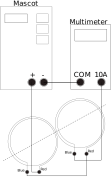
\includegraphics[width=0.8\textwidth]{fig/circuit_double_coil}
    % \setlength{\unitlength}{0.4mm}
    % \begin{picture}(120,10)(20,0)
    %     \newsavebox{\OneCoil}
    %     \savebox{\OneCoil}(60,60)[l]{
    %     %\put(30,5){\line(1,0){88}}
    %     %\put(118,5){\line(0,1){23}}
    %     \put(114,32){\line(0,-1){26.5}}
    %     \put(118,28){\line(0,-1){37.5}}
        
    %     %\put(30,5){\line(0,1){14}}
    %     \qbezier(118, 28)(124, 28)(129,35)
    %     \qbezier(129, 35)(132, 40)(132,45)
    %     \qbezier(132,45)(132, 52)(125,58)
    %     \qbezier(125,58)(117, 63)(108,58)
    %     \qbezier(108,58)(102, 54)(101,45)
    %     \qbezier(101,45)(101, 38)(105,34.5)
    %     \qbezier(105,34.5)(109, 30)(115,30)
    %     %\color{red}
    %     \qbezier(115,30)(126, 31)(129,40)
    %     \qbezier(129,40)(132, 55)(118,58)
    %     \qbezier(118,58)(105, 59)(103,45)
    %     \qbezier(103,45)(102, 35)(114,32)
    %     }
    %     %%Single Coil begins
    %     \put(30,5){\line(1,0){123}}
    %     %\put(118,5){\line(0,1){23}}
    %     \put(118,20){\line(1,0){31}}
    %     \put(118,28){\line(0,-1){7}}
        
    %     \put(30,5){\line(0,1){14}}
    %     \qbezier(118, 28)(124, 28)(129,35)
    %     \qbezier(129, 35)(132, 40)(132,45)
    %     \qbezier(132,45)(132, 52)(125,58)
    %     \qbezier(125,58)(117, 63)(108,58)
    %     \qbezier(108,58)(102, 54)(101,45)
    %     \qbezier(101,45)(101, 38)(105,34.5)
    %     \qbezier(105,34.5)(109, 30)(115,30)
    %     %\color{red}
    %     \qbezier(115,30)(126, 31)(129,40)
    %     \qbezier(129,40)(132, 55)(118,58)
    %     \qbezier(118,58)(105, 59)(103,45)
    %     \qbezier(103,45)(102, 35)(114,32)
    %     \put(90,6.5){\Large$\longrightarrow$}%
    %     \put(103,6.5){\large$I$}%
        
    %     \put(50,15){\framebox(15,25)}%Multimeter
    %     \put(52.5,32){\framebox(10,5)}%Multimeter display
    %     \put(56,20){\circle{3}}%
    %     \put(55,18.7){\small$\bullet$}%
    %     \put(62,20){\circle{3}}%
    %     \put(60.7,18.7){\small$\bullet$}%
        
    %     \put(61.5,20){\line(1,0){53}}
    %     \put(114,32){\line(0,-1){12}}
    %     \put(52,16){\tiny\sf COM}%
    %     \put(45,45){\sf Multimeter}%
    %     %\color{red}
    %     \put(114,20){\circle{3}}%
    %     \put(113,18.7){\small$\bullet$}%
    %     \put(118,20){\circle{3}}%
    %     \put(116.7,18.7){\small$\bullet$}%
    %     \put(105,22){\sf Bl\aa}%
    %     \put(119,22){\sf R\o d}%
    %     %\color{green}
    %     %%%%%%%%%Mascot begins
    %     \put(20,15){\framebox(20,34)}%Mascot
    %     \put(22,40){\framebox(9,5)}%Mascot
    %     \put(35,43){\framebox(3,5)}%Mascot
    %     \put(35,36){\framebox(3,5)}%Mascot
    %     \put(35,29){\framebox(3,5)}%Mascot
    %     \put(30,20){\circle{3}}%
    %     \put(28.8,18.7){\small$\bullet$}%
    %     \put(36,20){\circle{3}}%
    %     \put(34.6,18.7){\small$\bullet$}%
    %     \put(28,23){$+$}%
    %     \put(34,23){$-$}%
    %     \put(35,20){\line(1,0){22}}%Mascot-to-Multimeter
    %     \put(23,54){\sf Mascot}%
    %     %%%%%%%%%Mascot ends
    %     %\color{green}
    %     \put(35,10){\usebox{\OneCoil}}
    %     %\color{red}
    %     \put(149,30){\circle{3}}%
    %     \put(148,28.7){\small$\bullet$}%
    %     \put(153,30){\circle{3}}%
    %     \put(151.7,28.7){\small$\bullet$}%
    %     \put(140,32){\sf Bl\aa}%
    %     \put(154,32){\sf R\o d}%
    %     %\qbezier(90,32)(128, 51)(166,70)
    %     %\put(90,30){\line(2,1){22}}
    %     \multiput(86,30)(14,7){6}{\line(2,1){12}}
    %     %\put(90,70){\dashbox{0.2}(40,10)}%upper rectangle
    % \end{picture}
    \caption{%
        The Helmholtz coil circuit.
        Note that for the coils to be sufficiently close, the coils must be mounted with the connectors pointing out.
        Take care to have the current flow in the same direction in each coil.
    }
    \label{magnetfelt.fig7}
\end{marginfigure}
    \item Measure the magnetic field $B(x)$ along the coil axis as a function of the distance $x$ from the center plane between the coils with e.g. $I = \SI{1.00}{\ampere}$ and enter the results in the spreadsheet table for the Helmholtz coil. Continue some distance outside the end of the spool.
    \item Repeat the measurement with coil distances $a = 2R$ and $a = R/2$.
    \item Analyze the results and compare measured and calculated value. Print out the table and graph, and paste in the journal.
\end{itemize}


\subsection{Magnetic field in Anti-Helmholtz coil}
%%%%%%%%%%%%%%%%%%%%%%%%%%%%%%%%%%%%%

Task:
\emph{Repeat the same experiment as above for Anti-Helmholtz coils.}

\subsection{Magnetic field in solenoid}
%%%%%%%%%%%%%%%%%%%%%%%%%%%%%%%%%%%%%

Task:
\emph{Investigate the magnetic field along the axis of a solenoid.}

\textbf{Procedure:}
\begin{itemize}
    \item Mount the solenoid on the movable carriage and connect the circuit.
    \item Measure the magnetic field $B(x)$ along the axis of the solenoid as a function of the distance $x$ from the end plane of the solenoid, and enter the results in the spreadsheet.
    \item Analyze the results and compare measured and calculated value. Print out the table and graph, and paste in the journal.
\end{itemize}

\subsection{Magnetic field in short coil - extra assignment}
%%%%%%%%%%%%%%%%%%%%%%%%%%%%%%%%%%%%%

Task:
\emph{Investigate the magnetic field parallel to a short coil ($y$-axis) as a function of the distance from the coil.}
 
%Drøfting av måleprosedyren: 

Here the coil is mounted so that the magnetic field sensor passes parallel to the coil. How does the field vary? (Take note of the direction of the field.) Explain why the curve looks the way it does.

\subsection{General Discussion}
%%%%%%%%%%%%%%%%%%%%%%%%%%%%%%%%%%%%%

\begin{itemize}
   \item Carry out error analysis of the results and discuss possible systematic deviations.
   \item Discuss discrepancies between measurement results and the modeling you have included in the calculation section. Where are the biggest differences? What is the reason?
    %\item Diskuter bruken av høyrehåndsregelen.
    %\item Diskuter strøm- og spenningsregulering av kraftforsyninger.
    \item Discuss possible applications of the physical effects observed in the experiment.
\end{itemize}

%%%%%%%%%%%%%%%%%%%%%%%%%%%%%%%%%%%%%%%%%%%%%%%%%%
\subsection{Before you leave}
%%%%%%%%%%%%%%%%%%%%%%%%%%%%%%%%%%%%%%%%%%%%%%%%%%

Switch off all appliances, unplug all cables and leave the space in at least as good an order as you found it.

\end{document}


